\documentclass{article}
\usepackage{amsmath}
\usepackage{amssymb}
\usepackage{graphicx}
\usepackage{ctex}
\begin{document}
\title{第一次作业}
\maketitle
\begin{minipage}[b]{0.5\linewidth}
学号:190320517\\
姓名:葛旭\\
班级:自动化五班\\
\end{minipage}
\hfill
\begin{minipage}[b]{0.5\linewidth}
\includegraphics[width=0.45\textwidth]{gexu.eps}\\
\end{minipage}
1.B\\
2.D\\
3.B\\
4.C\\
5.C\\
6.D\\
7.\[\begin{gathered}
  A = 2 \times {10^{ - 2}}m,T = 1.0s \Rightarrow \omega  = 2\pi {\kern 1pt} {\kern 1pt} rad/s \hfill \\
  \phi  = \frac{{3\pi }}{4} \Rightarrow x = A\cos (\omega t + \phi ) = 0.02\cos (2\pi t + \frac{{3\pi }}{4}) \hfill \\
  v =  - 0.04\pi \sin (2\pi t + \frac{{3\pi }}{4}),a =  - 0.08{\pi ^2}\cos (2\pi t + \frac{{3\pi }}{4}) \hfill \\
  \left\{ \begin{gathered}
  x = 0.02\cos (2\pi t + \frac{{3\pi }}{4}) \hfill \\
  v =  - 0.04\pi \sin (2\pi t + \frac{{3\pi }}{4}) \hfill \\
  a =  - 0.08{\pi ^2}\cos (2\pi t + \frac{{3\pi }}{4}) \hfill \\
\end{gathered}  \right. \hfill \\
\end{gathered} \]
\begin{figure}[!h]\centering
\includegraphics[width=.9\textwidth]{9-7-x.eps}
\includegraphics[width=.9\textwidth]{9-7-v.eps}
\includegraphics[width=.9\textwidth]{9-7-a.eps}
\end{figure}\\
8.\[\begin{gathered}
  (1)A = 0.10m,\nu  = 10Hz,\omega  = 20\pi ,T = \frac{1}{{10}}s,\phi  = \frac{\pi }{4} \hfill \\
  (2)x = 0.10\cos (20\pi t + \frac{\pi }{4}) \hfill \\
   \Rightarrow v =  - 2\pi \sin (20\pi t + \frac{\pi }{4}) \hfill \\
   \Rightarrow a =  - 40{\pi ^2}\cos (20\pi t + \frac{\pi }{4}) \hfill \\
  t = 2s,x = \frac{{\sqrt 2 }}{{20}}m,v =  - \sqrt 2 \pi m/s,a =  - 20\sqrt 2 {\pi ^2}m/{s^2} \hfill \\
\end{gathered} \]
14.\[\begin{gathered}
  (1)A = 0.02m,\omega  = 4\pi ,\phi  = 0 \hfill \\
   \Rightarrow x = 0.02\cos (4\pi t) \hfill \\
  (2)A = 0.02m,\omega  = 4\pi ,\phi  = \frac{\pi }{2} \hfill \\
   \Rightarrow x = 0.02\cos (4\pi t + \frac{\pi }{2}) \hfill \\
  (3)A = 0.02m,\omega  = 4\pi ,\phi  = \frac{\pi }{3} \hfill \\
   \Rightarrow x = 0.02\cos (4\pi t + \frac{\pi }{3}) \hfill \\
  (4)A = 0.02m,\omega  = 4\pi ,\phi  = \frac{{4\pi }}{3} \hfill \\
   \Rightarrow x = 0.02\cos (4\pi t + \frac{{4\pi }}{3}) \hfill \\
\end{gathered} \]
15.\[\begin{gathered}
  (1) - kx + mg = ma \hfill \\
  \frac{{{d^2}x}}{{d{t^2}}} + \frac{k}{m}x = g \hfill \\
   \Rightarrow x = {c_1}\cos (t\sqrt {\frac{k}{m}} ) + {c_2}\sin (t\sqrt {\frac{k}{m}} ) + \frac{g}{{100}} \hfill \\
  {\text{from the question we know that }}\frac{k}{m} = 100 \hfill \\
   \Rightarrow x = {c_1}\cos (10t) + {c_2}\sin (10t) + \frac{g}{{100}} \hfill \\
  t = 0,\phi  = 0 \Rightarrow {c_2} = 0,{c_1} =  - 0.178 \hfill \\
  x =  - 0.178\cos (10t) + \frac{g}{{100}} \hfill \\
  (2)t = 0,x = 0.098m \hfill \\
  v =  - {c_1}\sqrt {\frac{k}{m}} \sin (t\sqrt {\frac{k}{m}} ) + {c_2}\sqrt {\frac{k}{m}} \cos (t\sqrt {\frac{k}{m}} ),v =  - 0.6m/s \hfill \\
  {c_1} = 0,{c_2} =  - 0.06 \hfill \\
  x =  - 0.06\sin (10t) + \frac{g}{{100}} \hfill \\
\end{gathered} \]
16.\[\begin{gathered}
  (1)A = 0.10,\phi  =  - \frac{\pi }{3},\omega t = \frac{{5\pi }}{6} \hfill \\
  t = 4s,\omega  = \frac{{5\pi }}{{24}}rad/s \hfill \\
  x = 0.1\cos (\frac{{5\pi }}{{24}}t - \frac{\pi }{3}) \hfill \\
  (2){\phi _p} = 0 \hfill \\
  (3)t = \frac{{\frac{\pi }{3}}}{\omega } = 1.6s \hfill \\
\end{gathered} \]
17.\[(1)\frac{T}{4}(2)\frac{T}{{12}}(3)\frac{T}{6}\]
18.\[\begin{gathered}
  \omega  = 4\pi ,A = 0.02m \hfill \\
  (1)mg - F = ma \hfill \\
  a =  - A{\omega ^2}\cos (\omega t + \phi ) \hfill \\
  mg + mA{\omega ^2}\cos (\omega t + \phi ) = F \hfill \\
  {\text{at the lowest point:}} \hfill \\
  \omega t + \phi  = 0 \hfill \\
  F = mg + mA{\omega ^2} = mg + mA{(\frac{{2\pi }}{T})^2} = 12.96N \hfill \\
  (2)mg + mA'{\omega ^2}\cos (\omega t + \phi ) = F,F = 0,\omega t + \phi  = \pi  \hfill \\
  mg = mA'{\omega ^2},A' = \frac{g}{{{\omega ^2}}} = 6.2 \times {10^{ - 2}}m \hfill \\
  (3)mg = mA\omega {'^2},\omega ' = \sqrt {\frac{g}{A}} ,\nu ' = \frac{{\omega '}}{{2\pi }} = \frac{1}{{2\pi }}\sqrt {\frac{g}{A}}  = 3.52Hz \hfill \\
\end{gathered} \]
20.\[x = A\cos (\omega t + \phi  - \frac{\pi }{2})\]
21.\[\begin{gathered}
  (1)A\omega  = 3,\omega  = 1.5,T = \frac{{2\pi }}{\omega } = 4.2s \hfill \\
  (2){a_{\max }} = A{\omega ^2} = 4.5 \times {10^{ - 2}}m/{s^2} \hfill \\
  (3){v_0} =  - A\omega \sin \phi  = \frac{{A\omega }}{2},{v_0} > 0, \hfill \\
  \phi  =  - \frac{{5\pi }}{6},x = 2\cos (1.5t - \frac{{5\pi }}{6}) \hfill \\
\end{gathered} \]
28.\[\begin{gathered}
  (1)A{\omega ^2} = 4,\omega  = 20rad/s,T = \frac{{2\pi }}{{20}} = \frac{\pi }{{10}}s \hfill \\
  (2){V_{\max }} = A\omega  = 0.2m/s \hfill \\
  E = \frac{1}{2}mV_{\max }^2 = 0.002J \hfill \\
  {E_k} = E \hfill \\
  (3)\frac{1}{2}k{x^2} = \frac{1}{4}k{A^2} \hfill \\
  x = \frac{{\sqrt 2 }}{2}A =  \pm 7.07 \times {10^{ - 3}} \hfill \\
  (4){E_p} = \frac{1}{2}k{x^2} = \frac{1}{2}k\frac{{{A^2}}}{4} = \frac{E}{4} = \frac{1}{2} \times {10^{ - 3}}J \hfill \\
  {E_k} = \frac{{3E}}{4} = \frac{3}{2} \times {10^{ - 3}}J \hfill \\
\end{gathered} \]
30.\[\begin{gathered}
  (1)\omega  = 8\pi ,T = \frac{{2\pi }}{\omega } = 0.25s \hfill \\
  A = 0.5m,\phi  = \frac{\pi }{3} \hfill \\
  (2)E = \frac{1}{2}k{A^2} = \frac{1}{2}m{\omega ^2}{A^2} = 7.9 \times {10^{ - 5}}J \hfill \\
  (3){E_k} = \frac{{\int_t^{t + T} {{E_k}dt} }}{T} = \frac{1}{4}k{A^2} = 3.95 \times {10^{ - 5}}J \hfill \\
  {E_p} = \frac{{\int_t^{t + T} {{E_p}dt} }}{T} = \frac{1}{4}k{A^2} = 3.95 \times {10^{ - 5}}J \hfill \\
\end{gathered} \]
\end{document}


